\renewcommand{\IMAGES}{../LAGR_POINT_SOURCE_DISPERSION/IMAGES}

\newcommand{\lra}[1]{\langle #1 \rangle }
\chapter{Lagrangian Point Source Dispersion}
\sousti{Christophe Henry, (INRIA Sophia Antipolis), Martin Ferrand, RENUDA}{27/07/20}
\keywords{3D, Lagrangian, Dispersion}
%--------------------------------------------------------------------------------------------------
\label{LAGR:case:lagr_point_source_dispersion}
%--------------------------------------------------------------------------------------------------
%%%%%%%%%%%%%%%%%%%%%%%%%%%%%%%%%%%%%%%%%%%%%%%%%%%%%%%%%
%                                                       %
%            Start of test case description             %
%                                                       %
%%%%%%%%%%%%%%%%%%%%%%%%%%%%%%%%%%%%%%%%%%%%%%%%%%%%%%%%%
%-----------------------------------

This test case corresponds to a verification case for the Lagrangian module in \CS.
It consists of point source dispersion.

\section{Description of the test case}
%-----------------------------------
\subsection{Introduction}
%........................
This test case consists in a fluid at rest in a cubic mesh (no flow) inside which particles are initially injected  in the centre of the domain.

To verify the present algorithm for the treatment of the equations of particle motion, numerical results are compared to analytical results in ideal cases that correspond to limiting cases (with constant coefficients).

This test case consists in an isotropic case as the one described in \cite{Rep1} and \cite{Rep2}: constant coefficients $C_i(t,\mathbf{x}_p) = 0$, $\mathbf{A}_i(t,\mathbf{x}_p) = 0$ and initial conditions $x_p(0)=U_p(0)=U_s(0)=0$.
In that case, the system simplifies to
\begin{equation} \label{eq:lagr:num_schem:syst}
\left\{\begin{aligned}
& dx_p = U_p\, dt \\
& dU_p = \frac{1}{\tau_p}(U_s-U_p)\, dt \\
& dU_s = -\frac{1}{T}U_s\,dt + \sigma\, dW(t),
\end{aligned}\right.
\end{equation}
and the solution of the system is
\begin{equation} \label{eq:lagr:num_schem:solved}
\left\{\begin{aligned}
& x_p = \Omega(t) \\
& U_p = \Gamma(t) \\
& U_s = \gamma(t),
\end{aligned}\right.
\end{equation}

%add yeude
The present test case was updated compared to the one detailed in \cite{Rep2}. Previously, the particles were injected at an inlet face and then displaced to the centre.  This led to having a combination of 5 symmetry boundary conditions and one inlet boundary condition.  Here, the particles are injected directly in the cell, which makes it possible to impose symmetry boundary conditions on all the cell faces and leads to slightly better results.
%end add yeude

\subsection{Theory}
The dynamics of discrete particles and the corresponding system of SDEs has been described in details in \cite{Rep3} and only the main features are recalled here. The system of SDEs describing the dynamics of the discrete particles reads
\begin{equation}
\left\{
\begin{aligned} \label{eq:lagr:num_scheme:sysEDS}
dx_{p,i}(t) & = U_{p,i}\, dt, \\
dU_{p,i}(t) & =\frac{1}{\tau_p}(U_{s,i}-U_{p,i})\, dt + \mathcal{A}_i\,dt,\\
dU_{s,i}(t) & =-\frac{1}{T_{L,i}^*}U_{s,i}\,dt+C_i\, dt + \sum_j
B_{ij}\, dW_j(t),
\end{aligned} \right .
\end{equation}
where $C_i$ is a term that includes all mean contributions: the mean pressure gradient, $-(\partial \lra{P}/\partial x_i)/\rho_f$, the mean drift term, $(\lra{U_{p,j}}-\lra{U_j})(\partial \lra{U_i}/\partial x_j)$, and the mean part of the return-to-equilibrium term, $\lra{U_i}/T^*_{L,i}$. $\mathcal{A}_i$ is an acceleration (gravity in the present work, but it can be extended for practical reasons to the case of other external force fields).

The weak numerical schemes, with the required features, are developed based on the analytical solution to Eqs.~(\ref{eq:lagr:num_scheme:sysEDS}) {\it with constant coefficients} (independent of time), the main idea being to derive a numerical scheme by freezing the coefficients on the integration intervals. This methodology ensures \textit{stability} and \textit{consistency with all limit systems}:
\begin{enumerate}
\item[-] stability because the form of the equations gives analytical solutions with exponentials of the type $\exp(-\Delta t/T)$ where $T$ is one of the characteristic timescales ($\tau_p$ and $T_{L,i}^*$),
\item[-] consistency with all limit systems by construction, since the schemes are based on an analytical solution.
\end{enumerate}
Different techniques shall be used to derive first and second-order (in time) schemes from the analytical solutions with constant coefficients. A first-order scheme can be obtained by computing, at each time step, the variables on the basis of the analytical solutions (all coefficients are frozen at the beginning of the integration interval), i.e. a numerical scheme of the {\it Euler} kind is obtained. A second-order scheme can be derived by resorting to a predictor-corrector technique where the prediction step is the first-order scheme.

\paragraph{Analytical solution} Before presenting the weak numerical schemes, it is a prerequisite to give the analytical solutions to system (\ref{eq:lagr:num_scheme:sysEDS}), with constant coefficients (in time). These solutions are obtained by resorting to It\^o's calculus in combination with the method of the variation of the constant. For instance, for the fluid velocity seen, one seeks a solution of the form $U_{s,i}(t)=H_i(t)\exp(-t/T_i)$, where $H_i(t)$ is a stochastic process defined by (\textit{from now on the notation is slightly changed: $T_{L,i}^*$ is noted $T_i$ for the sake of clarity in the complex formulae to come})
\begin{equation} \label{eq:H}
dH_i(t)=\exp(t/T_i)[C_i\,dt + \Check{B}_i\,dW_i(t)],
\end{equation}
that is, by integration on a time interval $[t_0,t]$ ($\Delta t=t-t_0$),
\begin{equation}
\begin{split}
U_{s,i}(t) = U_{s,i}(t_0)& \exp(-\Delta t/T_i)+ C_i
             \,T_i\,[1-\exp(-\Delta t/T_i)] \\
+ & \Check{B}_i \exp(-t/T_i)
    \int_{t_0}^{t}\exp(s/T_i)\,dW_i(s),
\end{split}
\end{equation}
where $\Check{B}_i=B_{ii}$ since $B_{ij}$ is a diagonal matrix). By proceeding in the same way for the other equations (position and velocity), the analytical solution is obtained for the entire system, cf. Table \ref{tab:lagrangian:exa}. The three stochastic integrals, Eqs. (\ref{eq:lagr:num_scheme:gamma_exa}) to (\ref{eq:lagr:num_scheme:Omega_exa}) in Table \ref{tab:lagrangian:exa}, are centred Gaussian processes. These integrals are defined implicitly, but they can be simplified by integration by parts, cf. Table \ref{tab:lagrangian:exa}.

\begin{table}[htbp]
\caption{Analytical solutions to system (\ref{eq:lagr:num_scheme:sysEDS}) for time-independent coefficients.}
\hrule
\begin{align}
& x_{p,i}(t) = x_{p,i}(t_0)
  + U_{p,i}(t_0)\tau_p  [1-\exp(-\Delta t/\tau_p)]
  + U_{s,i}(t_0)\,\theta_i \{T_i[1-\exp(-\Delta t/T_i)] \notag \\
&  \hspace*{5mm} + \tau_p[\exp(-\Delta t/\tau_p)-1]\}
  + [C_i\,T_i]
    \{\Delta t-\tau_p[1-\exp(-\Delta t/\tau_p)] \notag \\
&  \hspace*{5mm} - \theta_i (T_i[1-\exp(-\Delta t/T_i)]+
      \tau_p[\exp(-\Delta t/\tau_p)-1])\}
     + \Omega_i(t) \label{eq:lagr:num_scheme:xpa_exa} \\
&  \hspace*{5mm} \text{\quad with \quad} \theta_i = T_i/(T_i-\tau_p)
  \notag \\
& U_{p,i}(t) = U_{p,i}(t_0)\exp(-\Delta t/\tau_p)
  + U_{s,i}(t_0)\,\theta_i
    [\exp(-\Delta t/T_i)-\exp(-\Delta t/\tau_p)] \notag \\
& \hspace*{5mm} + [C_i\,T_i]
    \{[1-\exp(-\Delta t/\tau_p)]-\theta_i
      [\exp(-\Delta t/T_i)-\exp(-\Delta t/\tau_p)]\} \notag \\
& \hspace*{5mm} + \Gamma_i(t) \label{eq:lagr:num_scheme:Upa_exa} \\
& U_{s,i}(t) = U_{s,i}(t_0)\exp(-\Delta t/T_i)
  + C_i\,T_i[1-\exp(-\Delta t/T_i)]
  + \gamma _i(t) \label{eq:lagr:num_scheme:Ufa_exa} \\ \notag \\
%------------
& \text{\underline{The stochastic integrals $\gamma _i(t),\;\Gamma
_i(t),\;\Omega _i(t)$ are given by:}}\notag \\
& \quad \gamma _i(t) = \Check{B}_i\exp(-t/T_i)
  \int _{t_0}^{t} \exp(s/T_i)\,dW_i(s), \label{eq:lagr:num_scheme:gamma_exa}\\
& \quad \Gamma _i(t) = \frac{1}{\tau_p}\exp(-t/\tau_p)
  \int _{t_0}^{t}\exp(s/\tau_p)\,\gamma _i(s)\,ds, \label{eq:lagr:num_scheme:Gamma_exa}\\
& \quad \Omega _i(t) = \int _{t_0}^{t}\Gamma
_i(s)\,ds. \label{eq:lagr:num_scheme:Omega_exa} \\ \notag \\
%------------
& \text{\underline{By resorting to stochastic integration by parts, $\gamma
_i(t),\;\Gamma _i(t),\;\Omega _i(t)$ can be written:}}\notag \\
& \quad \gamma _i(t) = \Check{B}_i\,\exp(-t/T_i)
\,I_{1,i}, \label{eq:lagr:num_scheme:gammaN_exa}\\
& \quad \Gamma _i(t) = \theta_i \,\Check{B}_i\,
 [\exp(-t/T_i)\,I_{1,i} -\exp(-t/\tau_p)\,I_{2,i}], \label{eq:lagr:num_scheme:GammaN_exa}\\
& \quad \Omega _i(t) = \theta_i \,\Check{B}_i\,
   \{ (T_i-\tau_p)\,I_{3,i} \notag \\
& \hskip 4.0cm -[T_i \exp(-t/T_i)\,I_{1,i} -
   \tau_p \exp(-t/\tau_p) \,I_{2,i}]\}, \label{eq:lagr:num_scheme:OmegaN_exa} \\
& \text{with} \quad I_{1,i} = \int_{t_0}^{t}\exp(s/T_i)\,dW_i(s),
\quad I_{2,i}= \int_{t_0}^{t}\exp(s/\tau_p)\,dW_i(s) \notag \\
& \hskip 7.5cm \text{and} \quad I_{3,i}=\int_{t_0}^{t}dW_i(s).\notag
\end{align}
\hrule
\label{tab:lagrangian:exa}
\end{table}

\paragraph{Weak first-order scheme} From the analytical solutions of this system assuming constant coefficients, the weak-first order scheme is extracted. The equations are described in Table~\ref{tab:lagrangian:sch1}.

\begin{table}[htbp]
\caption{Weak first-order scheme (Euler scheme)}
\hrule
\begin{align}
& \text{\underline{Numerical integration of the system:}}\notag \\
& \quad x_{p,i}^{n+1} = x_{p,i}^n + A_1\,U_{p,i}^n + B_1\,U_{s,i}^n
  + C_1\,[T_i^n C_i^n] + \Gamma _i^n,
  \notag \\
& \quad U_{p,i}^{n+1} = U_{p,i}^n\, \exp(-\Delta t/\tau_p^n)
              + D_1\,U_{s,i}^n + [T_i^n C_i^n](E_1-D_1)
              + \Omega _i^n, \notag \\
& \quad U_{s,i}^{n+1} = U_{s,i}^n\, \exp(-\Delta t/T_i^n)
              + [T_i^n C_i^n] [1-\exp(-\Delta t/T_i^n)]
              + \gamma _i^n.\notag \\ \notag \\
%----------------
& \text{\underline{The coefficients $A_1,\;B_1,\;C_1,\;D_1$ and $E_1$ are
  given by:}}\notag \\
& \quad A_1 = \tau_p^n\,[1-\exp(-\Delta t/\tau_p^n)],\notag\\
& \quad B_1 = \theta_i ^n\,[T_i^n(1-\exp(-\Delta t/T_i^n)-A_1]
      \quad \text{with}\quad \theta_i ^n = T_i^n/(T_i^n-\tau_p^n),\notag\\
& \quad C_1 = \Delta t - A_1 - B_1, \notag \\
& \quad D_1 = \theta_i ^n [\exp(-\Delta t/T_i^n)-\exp(-\Delta
  t/\tau_p^n)],\notag\\
& \quad E_1 = 1 - \exp(-\Delta t/\tau_p^n).\notag \\ \notag \\
%----------------
& \text{\underline{The stochastic integrals $\gamma _i^n,\;\Omega
_i^n,\;\Gamma_i^n$ are simulated by:}}\notag \\
& \quad \gamma_i^n = P_{11}\,{\mathcal G}_{1,i},\notag \\
& \quad \Omega_i^n = P_{21}\,{\mathcal G}_{1,i}+ P_{22}\,{\mathcal G}_{2,i} \notag \\
& \quad \Gamma_i^n = P_{31}\,{\mathcal G}_{1,i}+ P_{32}\,{\mathcal G}_{2,i}+
                     P_{33}\,{\mathcal G}_{3,i}, \notag\\
& \quad \text{where ${\mathcal G}_{1,i},\;{\mathcal G}_{2,i},\;{\mathcal G}_{3,i}$ are
  independent ${\cal N}(0,1)$ random variables.} \notag\\ \notag \\
%----------------
& \text{\underline{The coefficients
 $P_{11},\;P_{21},\;P_{22},\;P_{31},\;P_{32},\;P_{33}$ are defined
 as:}}\notag\\
& \quad P_{11} = \sqrt{\lra{(\gamma_i^n)^2}}, \notag \\
& \quad P_{21} = \frac{\lra{\Gamma_i^n\gamma_i^n}}{\sqrt{\lra{(\gamma_i^n)^2}}},
  \quad P_{22} = \sqrt{\lra{(\Gamma_i^n)^2}-
  \frac{\lra{\Gamma_i^n\gamma_i^n}^2}{\lra{(\gamma_i^n)^2}}},\notag \\
& \quad P_{31} = \frac{\lra{\Omega_i^n\gamma_i^n}}{\sqrt{\lra{(\gamma_i^n)^2}}},
  \quad P_{32} = \frac{1}{P_{22}}(\lra{\Omega_i^n\Gamma_i^n}-P_{21}P_{31}),
  \quad P_{33} = \sqrt{\lra{(\Omega_i^n)^2}-P_{31}^2-P_{32}^2)}.\notag
\end{align}
\hrule
\label{tab:lagrangian:sch1}
\end{table}

\paragraph{Weak second-order scheme} The weak second-order scheme consists in a corretion step for the particle velocity and the velocity of the fluid seen as described in Table~\ref{tab:lagrangian:sch2}:
\begin{table}[htbp]
\caption{Weak second-order scheme}
\hrule
\begin{align}
& \text{\underline{Prediction step:}}
\quad \text{Euler scheme, see Table \ref{tab:lagrangian:sch1} (predicted values noted with $\tilde{ }$ )} .\notag \\
%----------------
& \text{\underline{Correction step:}} \notag \\
& \quad U_{p,i}^{n+1} =
    \frac{1}{2}\,U_{p,i}^n\, \exp(-\Delta t/\tau_p^n)
  + \frac{1}{2}\,U_{p,i}^n\,\exp(-\Delta t/\tilde{\tau }_p^{n+1})\notag \\
& \qquad \qquad \qquad \qquad + \frac{1}{2}\,U_{s,i}^n\,C_{2c}(\tau_p^n,\,T_i^n)
  + \frac{1}{2}\,U_{s,i}^n\,C_{2c}(\tilde{\tau}_p^{n+1},\,\tilde{T_i}^{n+1})
\notag \\
& \qquad \qquad \qquad \qquad + A_{2c}(\tau_p^n,\,T_i^n) \,[T_i^n C_i^n]
  + B_{2c}(\tilde{\tau}_p^{n+1},\,\tilde{T}_i^{n+1})\,[\tilde{T}_i^{n+1} C_i^{n+1}]\notag \\
& \qquad \qquad \qquad \qquad + A_2(\Delta t,\tau_p^n)[\tau_p^n\,{\cal A}_i^n]
  + B_2(\Delta t,\tilde{\tau_p}^{n+1})[\tilde{\tau_p}^{n+1}\,{\cal A}_i^{n+1}]
  + \tilde{\Gamma}_i^{n+1}, \notag \\
& \quad U_{s,i}^{n+1} = \frac{1}{2}\,U_{s,i}^n\,\exp(-\Delta t/T_i^n)
+ \frac{1}{2}\,U_{s,i}^{n}\,\exp(-\Delta t/\tilde{T}_i^{n+1})
+ A_2(\Delta t,\,T_i^n) \,[T_i^n C_i^n]\notag \\
& \qquad \qquad \qquad \qquad
+ B_2(\Delta t,\,\tilde{T}_i^{n+1}) \,[\tilde{T}_i^{n+1} C_i^{n+1}]
+ \tilde{\gamma}_i^{n+1}.\notag\\
%----------------
& \text{\underline{The coefficients $A_2,\;B_2,\;A_{2c},\;B_{2c}$ et $C_{2c}$ are
  defined as:}}\notag \\
& \quad A_2(\Delta t,x) = -\exp(-\Delta t/x)
+ [1-\exp(-\Delta t/x)][x/\Delta t], \notag\\
& \quad B_2(\Delta t,x) = 1-[1-\exp(-\Delta t/x)][x/\Delta t],\notag \\
& \quad A_{2c}(x,y) =
- \exp(-\Delta t/x) + [(x+y)/\Delta t][1-\exp(-\Delta t/x)]
- (1+y/\Delta t)\,C_{2c}(x,y), \notag \\
& \quad B_{2c}(x,y) =  1 - [(x+y)/\Delta t][1-\exp(-\Delta t/x)]
+ (y/\Delta t)\,C_{2c}(x,y), \notag\\
& \quad C_{2c}(x,y) = [y/(y-x)][\exp(-\Delta t/y)-\exp(-\Delta
  t/x)].\notag \\
%----------------
& \text{\underline{The stochastic integrals
        $\tilde{\gamma}_i^{n+1}\;$ \text{and} $\;\tilde{\Gamma}_i^{n+1}$
        are simulated as follows:}}\notag \\
& \quad \tilde{\gamma}_i^{n+1}= \sqrt {\frac{[B_i^{*}]^2\tilde{T}_i^{n+1}}{2}
               [1-\exp(-2\Delta t/\tilde{T}_i^{n+1})]}\; {\mathcal G}_{1,i},\notag \\
& \quad \text{with} \quad \left[1-\exp(-2\,\Delta t/\tilde{T}_i^{n+1})\right]\,B_i^{*} =
    A_2(2\,\Delta t,\,\tilde{T}_i^{n+1})\,\sqrt{(\Check{B}_i^n)^2} + \notag \\
& \hskip 8.0cm B_2(2\,\Delta t,\,\tilde{T}_i^{n+1})\,\sqrt{(\tilde{\Check{B}}_i^{n+1})^2}. \notag \\
& \quad \tilde{\Gamma}_i^{n+1} =
  \frac{\lra{ \tilde{\Gamma}_i^{n+1}\tilde{\gamma}_i^{n+1} } }
     {\lra{(\tilde{\gamma}_i^{n+1})^2}}\,\tilde{\gamma}_i^{n+1}+
  \sqrt{\lra{(\tilde{\Gamma}_i^{n+1})^2}-
      \frac{\lra{\tilde{\Gamma}_i^{n+1}\tilde{\gamma}_i^{n+1}}^2}
           {\lra{(\tilde{\gamma}_i^{n+1})^2}} }\;{\mathcal G}_{2,i} \notag \\ \notag \\
& \quad \text{with}\quad \lra{ \tilde{\Gamma}_i^{n+1}\tilde{\gamma}_i^{n+1} } =
  \lra{\Gamma_i\gamma_i}(\tau_p^n,\,\tilde{T}_i^{n+1},\,B^{*}_i)
  \quad \text{and}\quad \lra{(\tilde{\Gamma}_i^{n+1})^2} =
  \lra{\Gamma_i^2}(\tau_p^n,\,\tilde{T}_i^{n+1},\,B^{*}_i). \notag
\end{align}
\hrule
\label{tab:lagrangian:sch2}
\end{table}

\clearpage

%add yeude
\subsection{References}

\begin{thebibliography}{3}

   \bibitem{Rep1} J.-P. Minier, E. Peirano, and S. Chibbaro. Weak first
   and second order numerical schemes for stochastic differential equations
   appearing in lagrangian two-phase flow modelling.
   {\it Monte Carlo Methods and Applications}, 9(2):93–133, 2003.

   \bibitem{Rep2} C. HENRY, J. POZORSKI
   Modelling of agglomeration and deposition of colloidal particles carried by a flow: Fourth progress report.
   {\it EDF Report}, Report-EDF-09-2016, 2016.
   
   \bibitem{Rep3} E. Peirano, S. Chibbaro, J. Pozorski, and J.-P. Minier.
   Mean-field/PDF numerical approach for polydispersed turbulent two-phase flows.
   {\it Progress in Energy and Combustion Science}, 32(3):315–371, 2006.

\end{thebibliography}

%end add yeude

\section{Numerical set up}
%-----------------------------------
\subsection{Computational domain}
%..............................
To perform a numerical simulation in such an ideal case, a very simple computational domain consisting of a single cubic cell (with a size of \SI{1000}{m}) has been retained.

\begin{figure}[H]
 \centering
 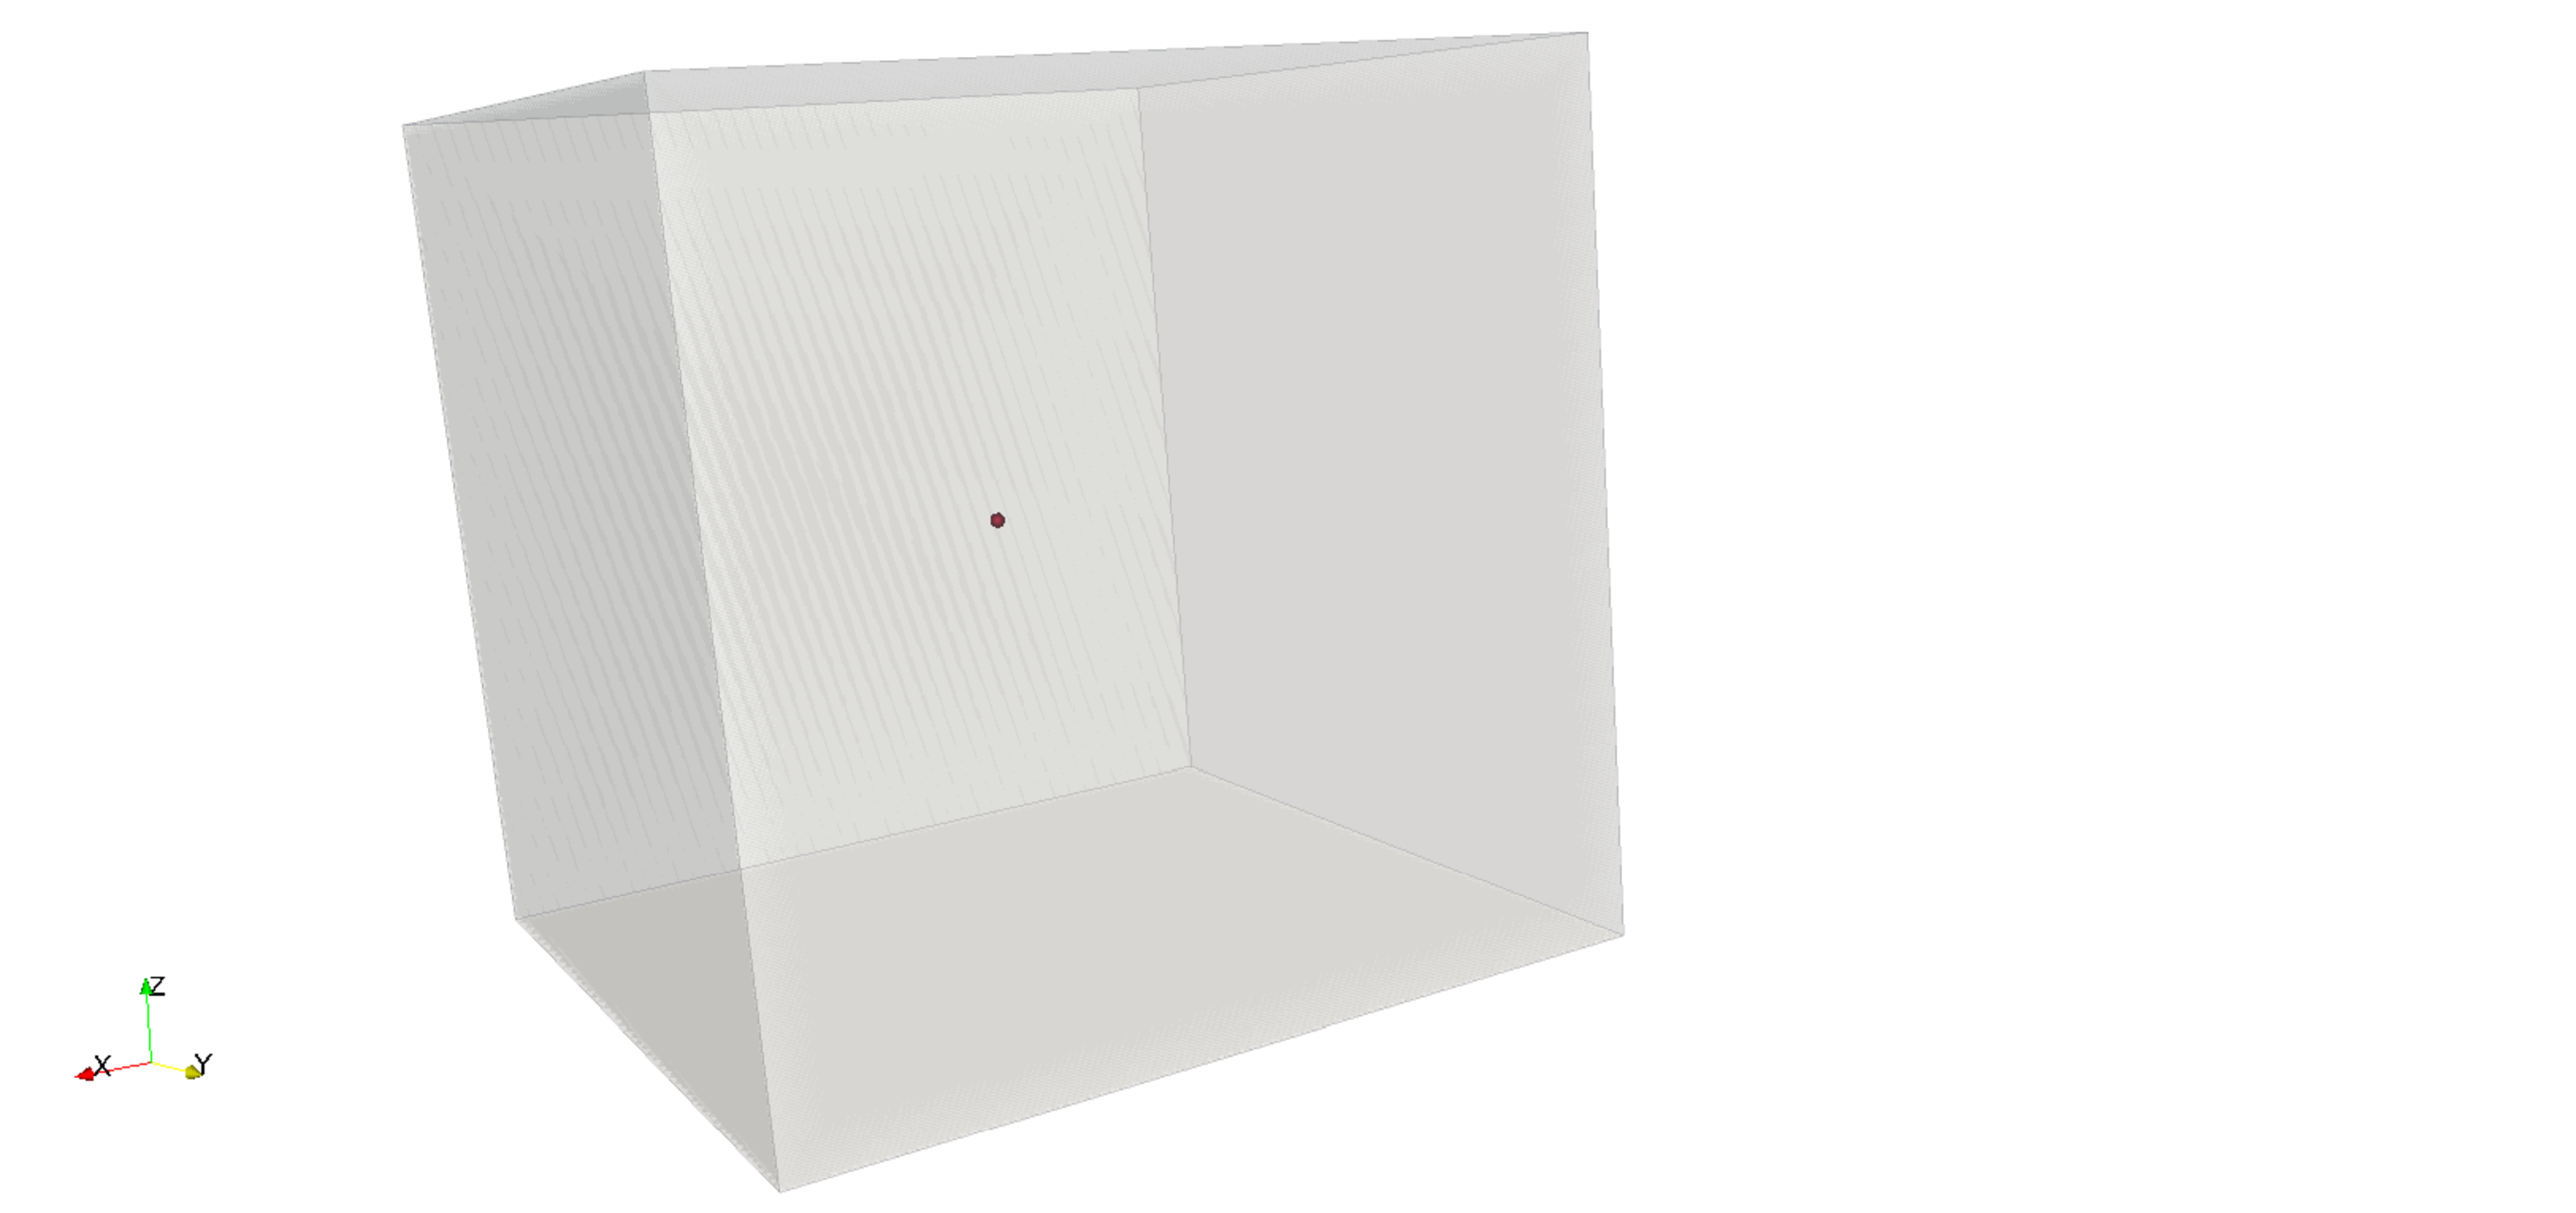
\includegraphics[scale=0.25, trim = 0cm 0cm 0cm 0cm, clip]{\IMAGES/Fig_NUM_SCHEME_mesh.pdf}
 \caption{3D view of the single cell used for the verification of the numerical scheme in ideal cases.}
 \label{Fig_NUM_SCHEME_Verif_mesh}
\end{figure}

%
\subsection{Physical modeling for the fluid flow}
%..............................
The fluid is at rest (no fluid motion).
Since all parameters are fixed manually in the Lagrangian module of \CS{}, the simulation of the fluid phase is not primordial. Nevertheless, the following parameters have been retained to be able to run a two-phase flow simulation. The flow is isothermal and incompressible. Gravity has been neglected. The properties used for the liquid in the flow domain are summarised in Table~\ref{Tab_NUM_SCHEME_fluid}:
\begin{table}[H]
\begin{center}
\begin{tabular}{|c|c|c|}
\hline
$U_{inlet}$ & $\mu_f$ 			& $\rho_f$ 		\\
\hline
\SI{0}{m.s^{-1}} & \SI{1.002e-3}{kg.m^{-1}.s^{-1}} 	& \SI{998}{kg.m^{-3}}	\\
\hline
\end{tabular}
 \caption{Fluid properties used in the simulation: inlet velocity $U_{inlet}$, Reynolds number $Re$, dynamic viscosity $\mu_f$ and density $\rho_f$.}
\label{Tab_NUM_SCHEME_fluid}
\end{center}
\end{table}

A turbulence model has been activated to be able to use the particle turbulent dispersion model:
\begin{itemize}
 \item Turbulence model: $k-\varepsilon$ (with initial values to get the desired Lagrangian times)
 \item Frozen dynamic field
\end{itemize}

\paragraph{Initial conditions}
\subparagraph{} The initial conditions are the following:
\begin{itemize}
 \item reference and initial pressure: \SI{101325}{Pa}
 \item fluid velocity: \SI{0.0}{m.s^{-1}}
 \item temperature: \SI{293.15}{K}
\end{itemize}

\paragraph{Boundary conditions}
%add yeude
%\subparagraph{Inlet boundary} An inlet boundary condition is needed for the particle injection. As a result, one of the faces of the cube is used as an inlet and the fluid is injected with the following properties:
%\begin{itemize}
% \item velocity: \SI{0.0}{m.s^{-1}}
% \item hydraulic diameter (for turbulence initialisation): \SI{1.0}{m}

%\subparagraph{Wall boundary} The other boundary conditions are fixed to symmetry.

%\end{itemize}

\subparagraph{} All the faces of the computational domain are defined as symmetry boundary conditions. The particles are injected directly at the centre of the computational domain.
%end add yeude

\subsection{Physical modelling for the particles}
%add yeude
%\subparagraph{Injection} Particles are injected in the domain at the inlet. The properties used for the injected particles are:
\subparagraph{Injection} Particles are injected in the domain. The properties used for the injected particles are:
%end add yeude
\begin{itemize}
 \item Particle diameter: \SI{1e-3}{m}
 \item Monodispersed particles
 \item Particle density: \SI{998}{kg.m^{-3}}
 \item Frequency of injection: 0 (only initially)
 \item Number of particles in class: \SI{20000}{}
\end{itemize}
%add yeude
%\subparagraph{Boundary condition} The wall boundary conditions for particles have been set to
\subparagraph{Boundary condition} The symmetry boundary conditions for particles have been set to
%end add yeude
\begin{itemize}
 \item symmetry (particles zero-flux)
\end{itemize}

\subparagraph{Model for transport} The CFD simulation with the injection of particles has been performed using the Lagrangian module in \textit{Code$\_$Saturne} and the following properties
\begin{itemize}
 \item Eulerian-Lagrangian multi-phase treatment: one way coupling
 \item The continuous phase is a steady flow
 \item No additional models associated with the particles
 \item Integration for the stochastic differential equations: first-order scheme or second-order scheme
 \item Particle turbulent dispersion model: activated
\end{itemize}
\subparagraph{Numerical parameters} The two-phase flow simulation has been performed using the following numerical parameters:
\begin{itemize}
 \item Calculation restart from the fluid flow simulation
 \item Constant time step: \SI{0.001}{s}
 \item Number of iterations: \SI{2000}{} or \SI{4000}{}
\end{itemize}

%add yeude
%The main subroutine of the Lagrangian module (cs\_lagr.c) has been modified to enforce fixed coefficients ($C_i(t,\mathbf{x}_p) = 0$, $\mathbf{A}_i(t,\mathbf{x}_p) = 0$, $T_L$, $\tau_p$) throughout the calculation while the injection (in cs\_lagr\_new.c) has also been modified to have all the particles starting from the middle of the simulation (see also Figure~\ref{Fig_NUM_SCHEME_Verif_mesh}). The various cases studied are summarised in Table~\ref{Tab_NUM_SCHEME_cases}:


The subroutines cs\_user\_initialization.c, cs\_user\_lagr\_particle.c, cs\_user\_lagr\_volume\_conditions.c, cs\_user\_mesh-modify.c are coded to set-up the test case.

\begin{description}

   \item[-] \textbf{cs\_user\_initialization.c} is used to initialize the turbulence $k$ and $eps$ from $T_L$ and $\sigma$. 
   \item[-] \textbf{cs\_user\_lagr\_volume\_conditions.c} is used to set-up the particle class. 
   \item[-] \textbf{cs\_user\_lagr\_particle.c} is used to set-up the parameter $\tau_p$ and to put all the particles at the middle of the domain (see also Figure~\ref{Fig_NUM_SCHEME_Verif_mesh}). 
   \item[-] \textbf{cs\_user\_mesh-modify.c} is used to center and scale the domain to \SI{1000}{m}.

\end{description}

The various cases studied are summarised in Table~\ref{Tab_NUM_SCHEME_cases}:

%end add yeude

\begin{table}[H]
\begin{center}
\begin{tabular}{|c|c|c|c|}
\hline
Case 		& $\tau_p$	 & $T_L$	& $\sigma$ 		\\
		& (s)		 & (s)		& (\SI{}{m.s^{-3/2}}) 	\\
\hline
 General case	& \SI{e-1}{} 	& \SI{2e-1}{}	& \SI{e1}{}	\\
\hline
 Limit case I	& \SI{e-5}{} 	& \SI{e-1}{}	& \SI{e1}{}	\\
\hline
 Limit case II	& \SI{e-1}{} 	& \SI{e-5}{}	& \SI{e3}{}	\\
\hline
 Limit case III	& \SI{2e-5}{} 	& \SI{e-5}{}	& \SI{e3}{}	\\
\hline
\end{tabular}
 \caption{Values of the fixed parameters in the various cases studied. General case: $\Delta t \ll T_L, \tau_p$. Limit case I: $\tau_p \ll \Delta t \ll T_L$. Limit case II: $T_L \ll \Delta t \ll \tau_p$. Limit case III: $\tau_p, T_L \ll \Delta t $.}
\label{Tab_NUM_SCHEME_cases}
\end{center}
\end{table}

%------------------------------------------
\section{Results}
%------------------------------------------

Two-phase flow simulations of system~\ref{eq:lagr:num_schem:syst} have been performed in the various cases previously mentioned. The system considered consists in purely diffusive motion of particles, as seen in Figure~\ref{Fig_NUM_SCHEME_Verif_part}.
\begin{figure}[H]
  \centering
  \subfigure[Zoom on the initial configuration]{
    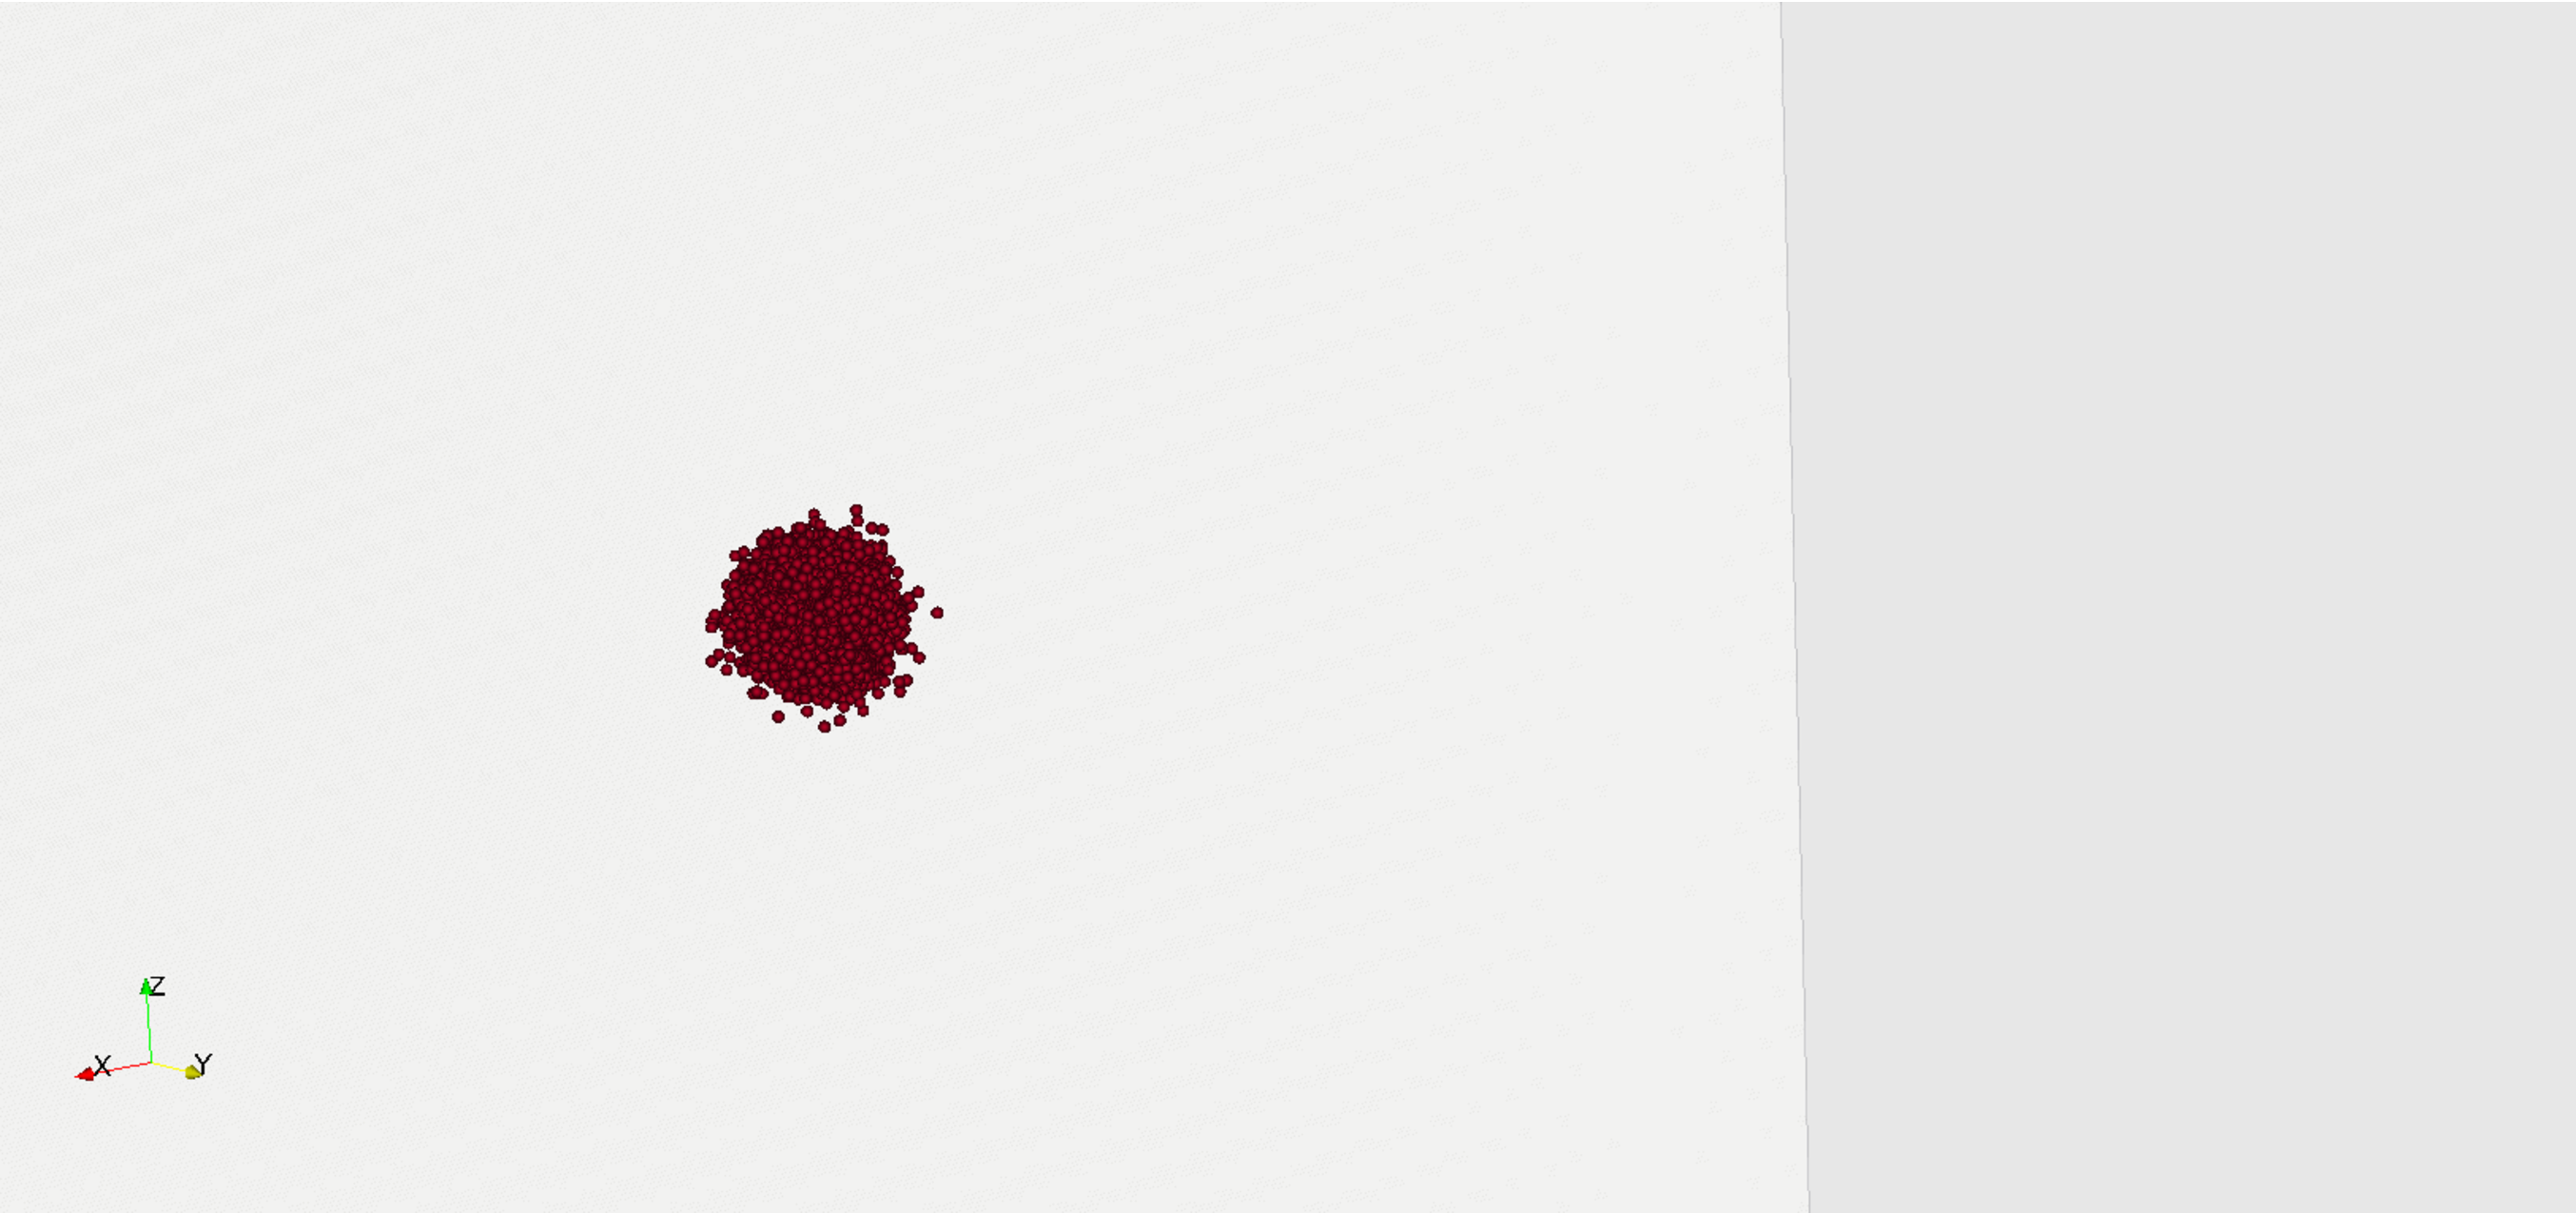
\includegraphics[width=0.48\textwidth, trim = 0cm 0cm 15cm 0cm, clip]{\IMAGES/Fig_NUM_SCHEME_part_init.pdf}
  }
  \subfigure[Zoom on the final configuration]{
    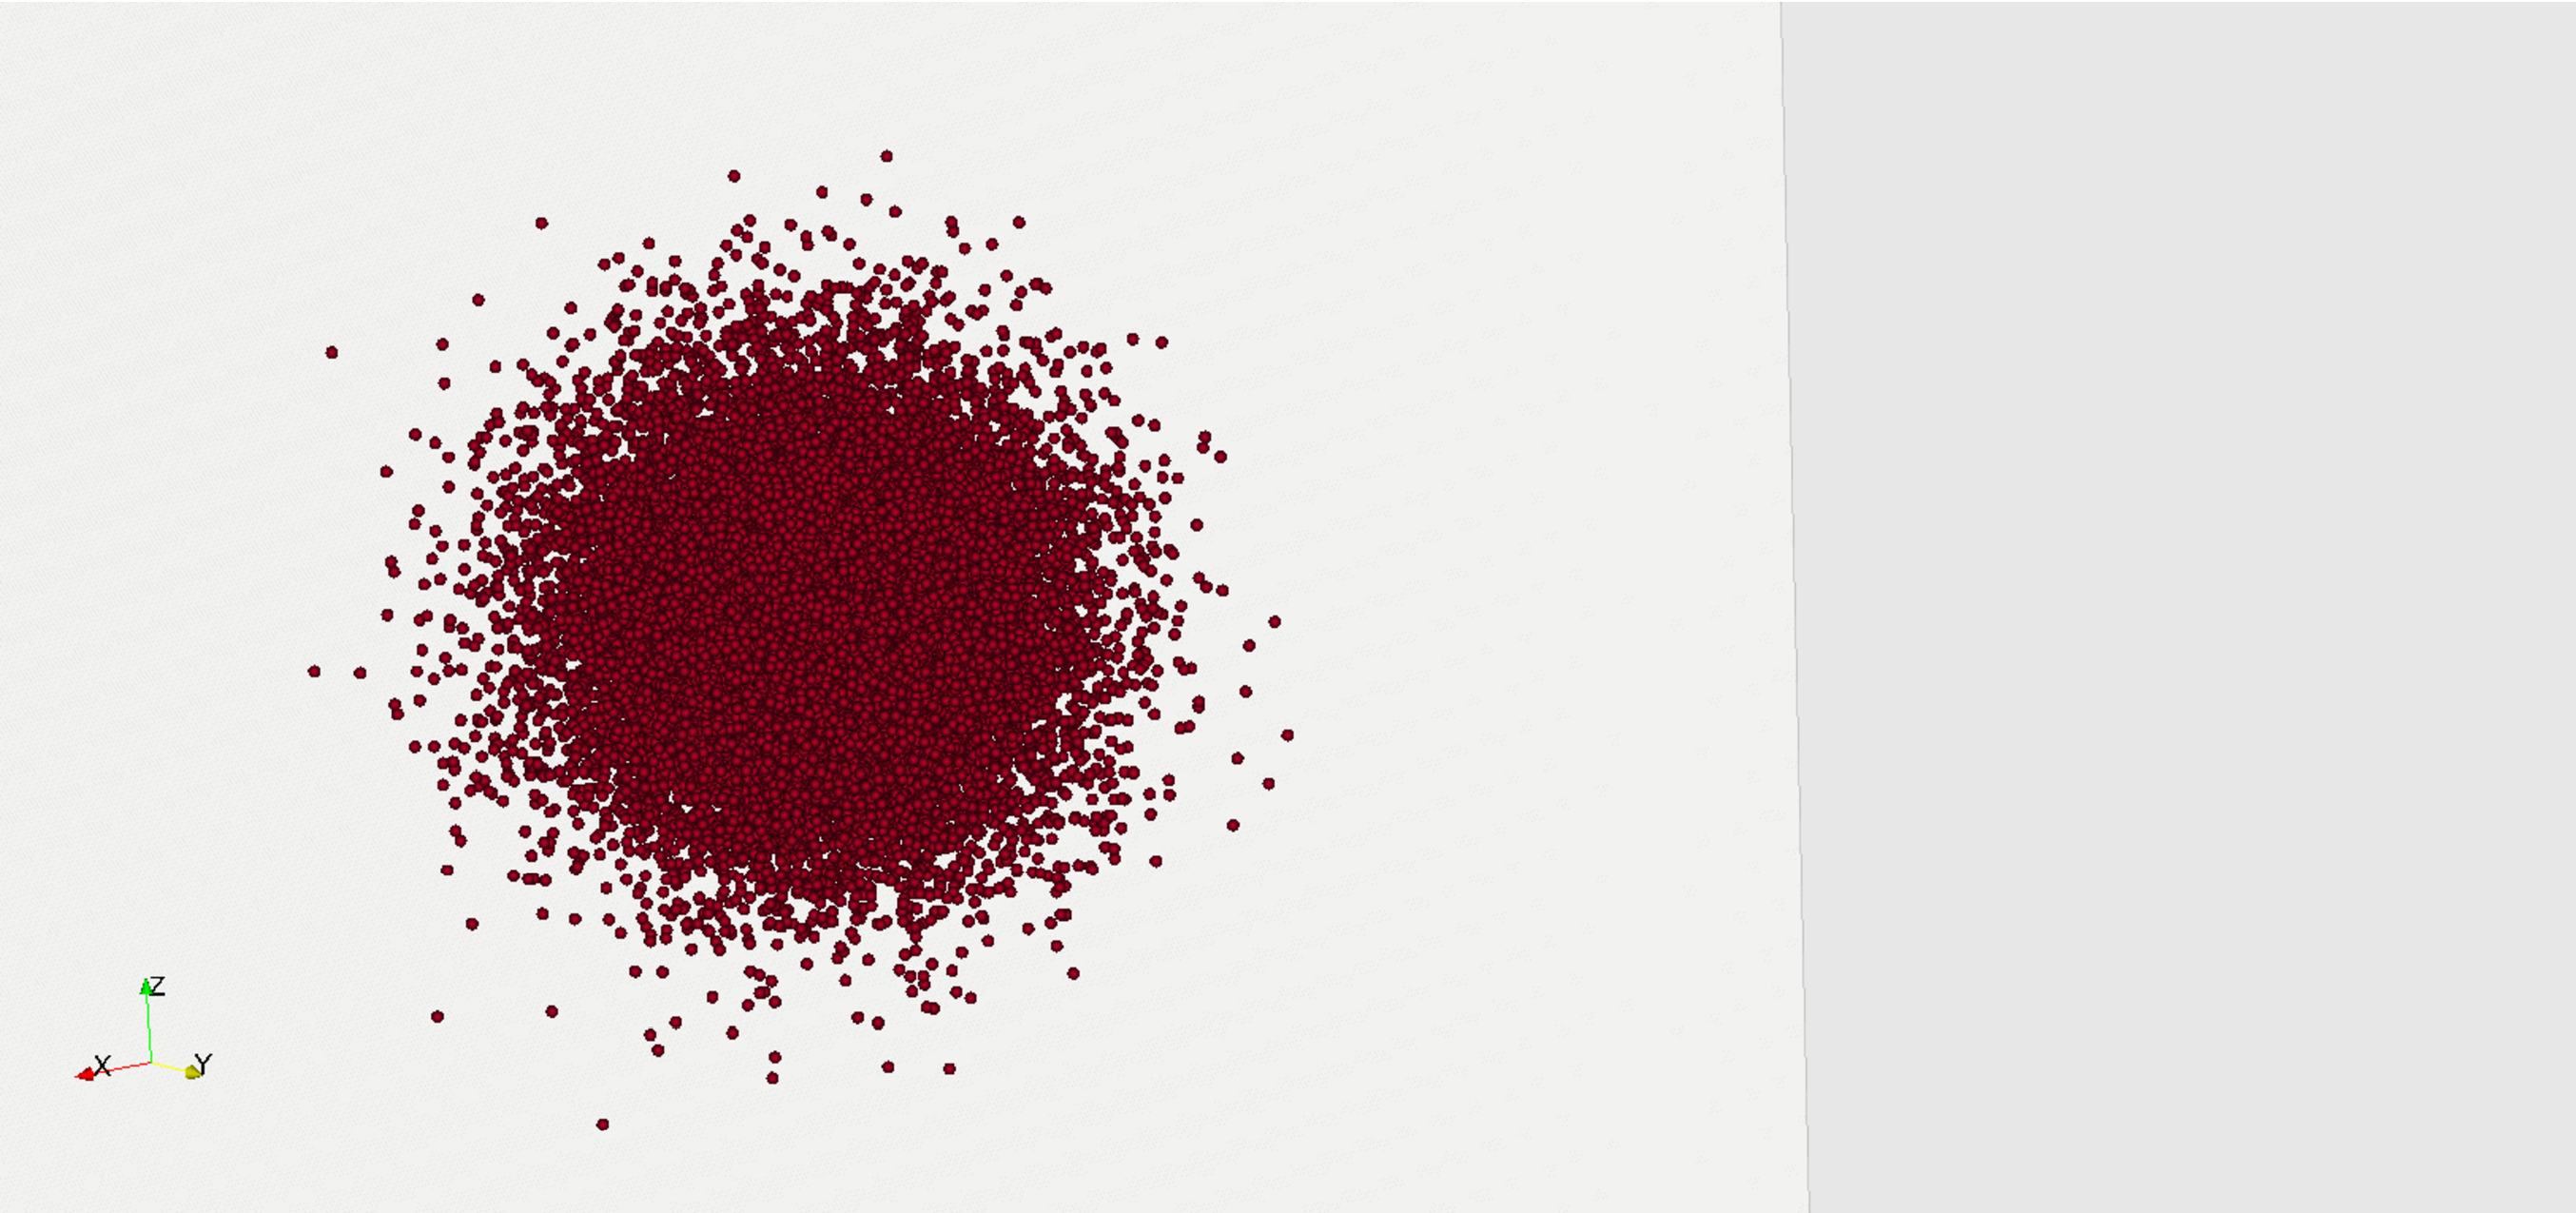
\includegraphics[width=0.48\textwidth,trim = 0cm 0cm 15cm 0cm, clip]{\IMAGES/Fig_NUM_SCHEME_part_end.pdf}
  }
  \caption{3D view of the particles inside single cell (zoom) at the initial and final time step.}
  \label{Fig_NUM_SCHEME_Verif_part}
\end{figure}

Results are displayed in Figures~\ref{Fig_NUM_SCHEME_GENERAL_CASE}-\ref{Fig_NUM_SCHEME_LIMIT_CASE_III} for the second-order moments (first-order moments are omitted since the solutions of system~\ref{eq:lagr:num_schem:syst} are Gaussian random variables with a mean equal to zero) in the various cases. It can be seen that all numerical results are close to the analytical solution.
\begin{figure}[H]
  \centering
  \subfigure[{Position}]{
    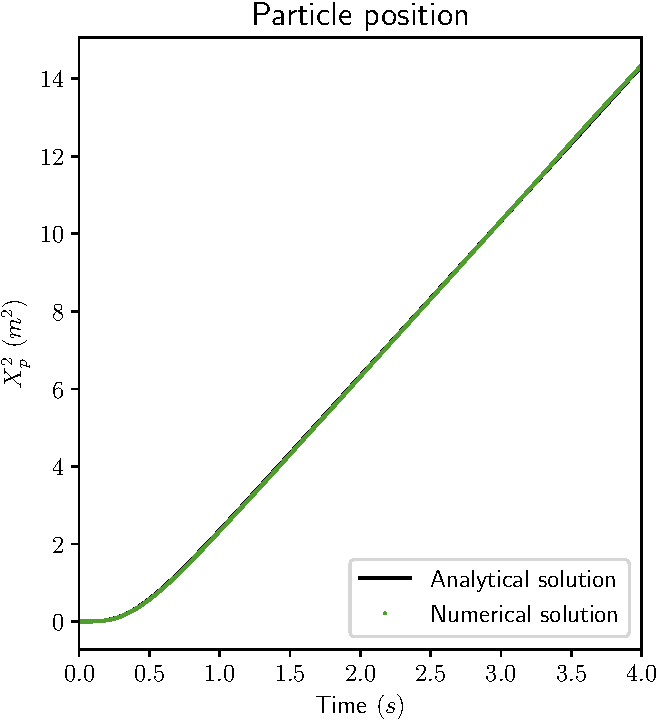
\includegraphics[width=0.48\textwidth]{\IMAGES/VNV/Fig_NUM_SCHEME_xp_xp_GENERAL_CASE.pdf}
  }
  \subfigure[{Particle velocity}]{
    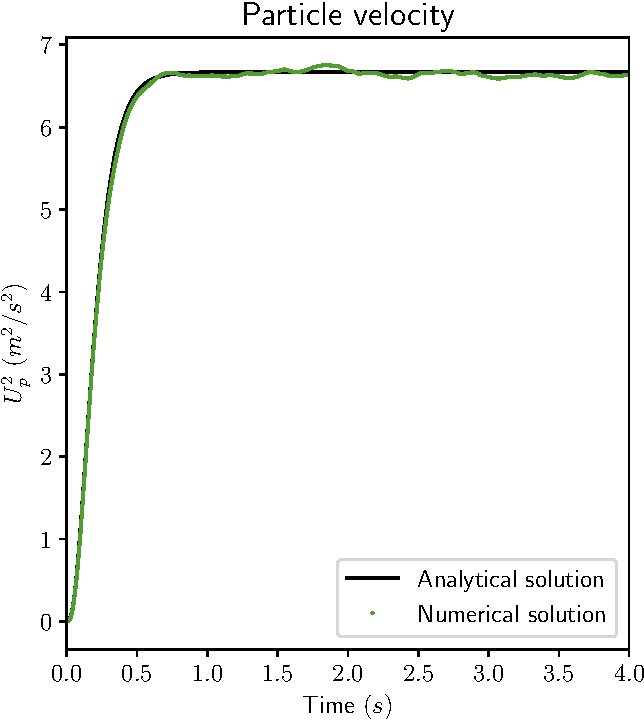
\includegraphics[width=0.48\textwidth]{\IMAGES/VNV/Fig_NUM_SCHEME_Up_Up_GENERAL_CASE.pdf}
  }
  \subfigure[{Fluid velocity seen}]{
    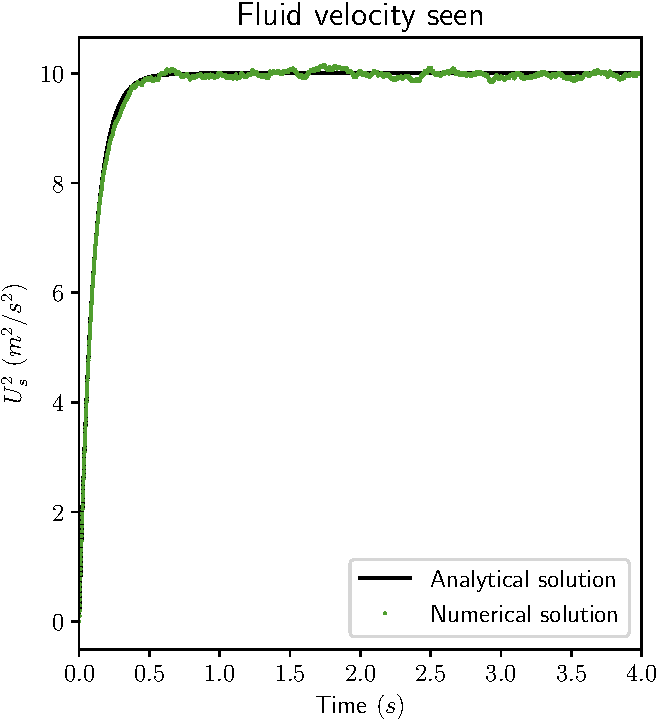
\includegraphics[width=0.48\textwidth]{\IMAGES/VNV/Fig_NUM_SCHEME_Us_Us_GENERAL_CASE.pdf}
  }
  \subfigure[{Velocity covariance}]{
    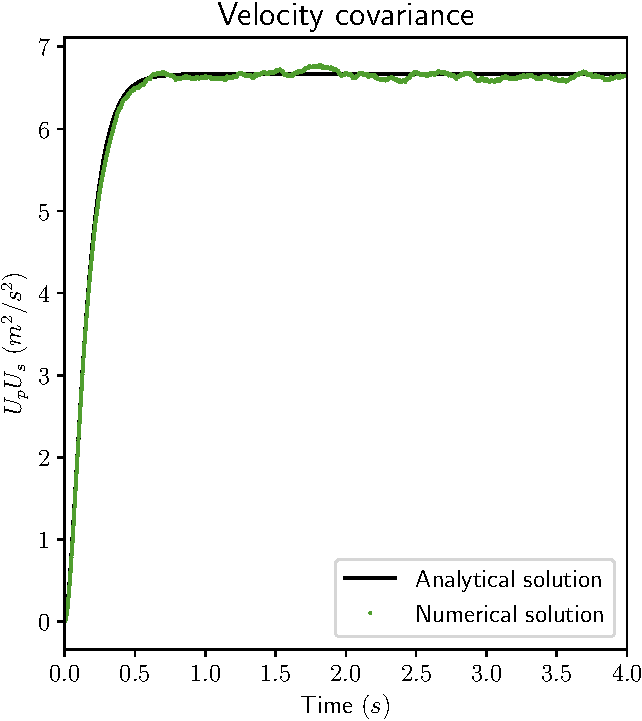
\includegraphics[width=0.48\textwidth]{\IMAGES/VNV/Fig_NUM_SCHEME_Up_Us_GENERAL_CASE.pdf}
  }
  \caption{Comparison of numerical results for system~\ref{eq:lagr:num_schem:syst} (symbols for $1^{st}$ and $2^{nd}$ order schemes) and analytical solutions (lines) in the general case.}
  \label{Fig_NUM_SCHEME_GENERAL_CASE}
\end{figure}

\begin{figure}[H]
  \centering
  \subfigure[{Position}]{
    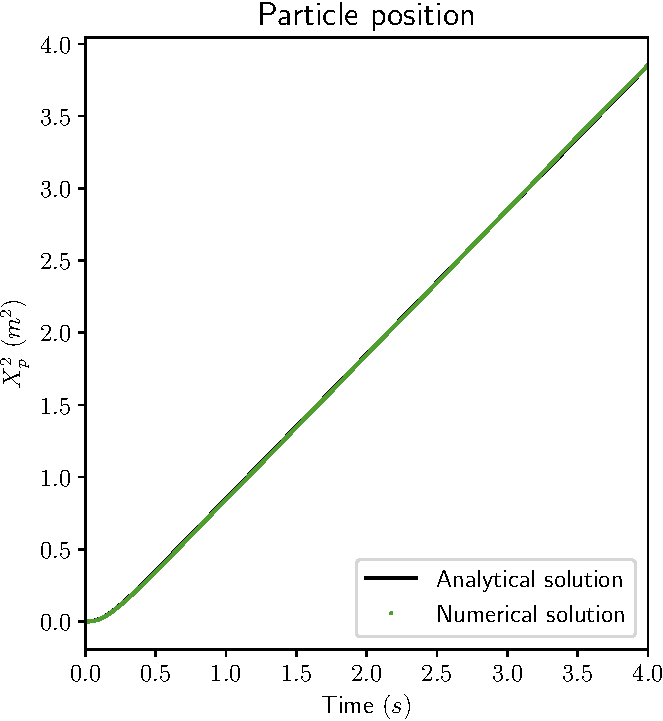
\includegraphics[width=0.48\textwidth]{\IMAGES/VNV/Fig_NUM_SCHEME_xp_xp_LIMIT_CASE_I.pdf}
  }
  \subfigure[{Particle velocity}]{
    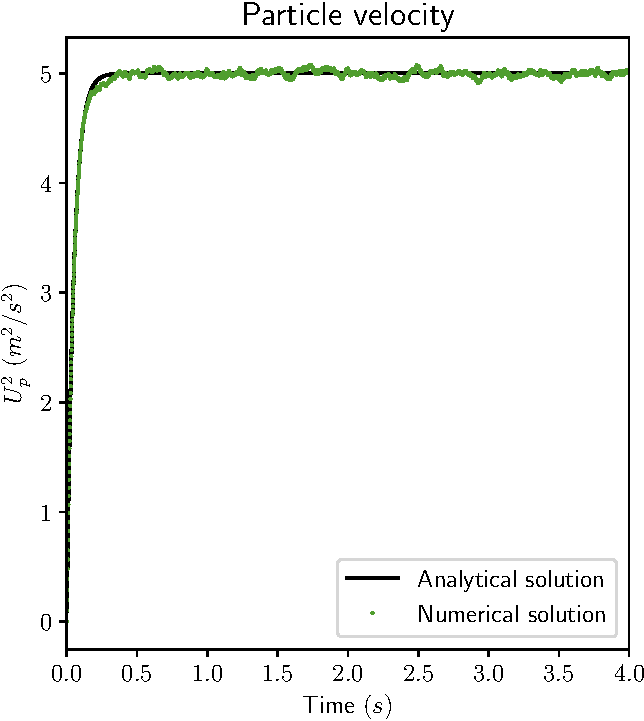
\includegraphics[width=0.48\textwidth]{\IMAGES/VNV/Fig_NUM_SCHEME_Up_Up_LIMIT_CASE_I.pdf}
  }
  \subfigure[{Fluid velocity seen}]{
    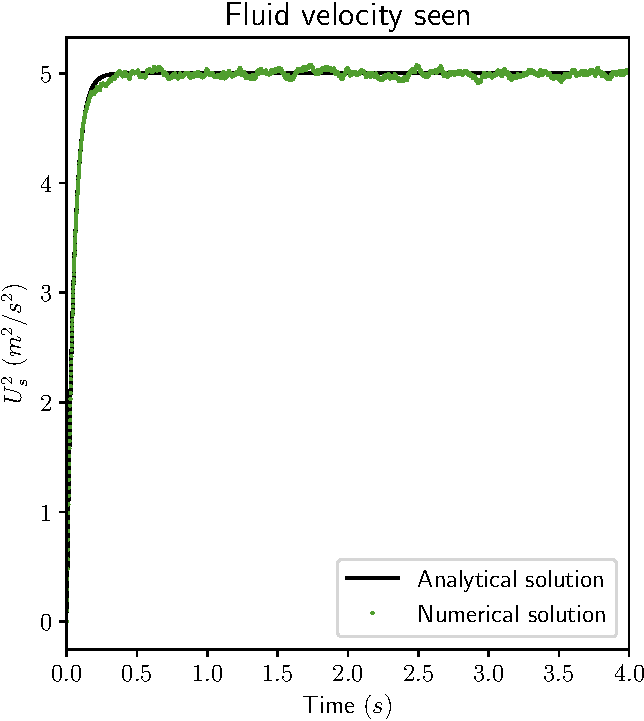
\includegraphics[width=0.48\textwidth]{\IMAGES/VNV/Fig_NUM_SCHEME_Us_Us_LIMIT_CASE_I.pdf}
  }
  \subfigure[{Velocity covariance}]{
    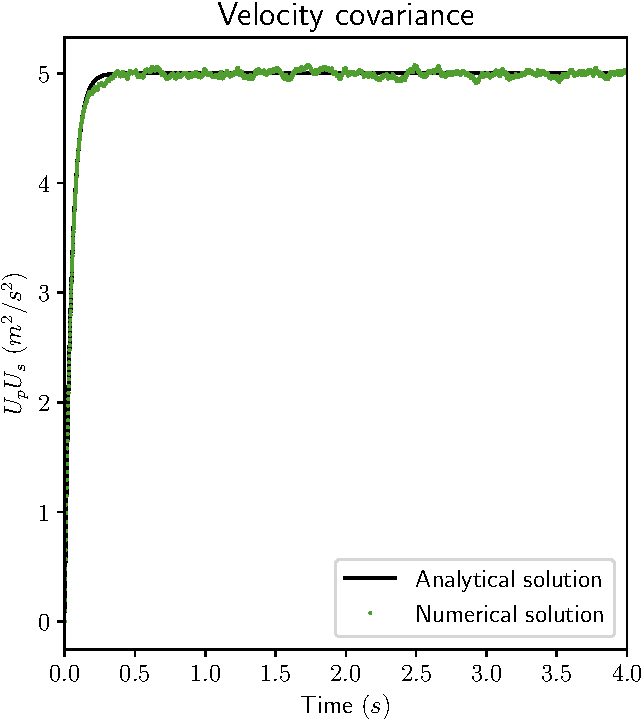
\includegraphics[width=0.48\textwidth]{\IMAGES/VNV/Fig_NUM_SCHEME_Up_Us_LIMIT_CASE_I.pdf}
  }
  \caption{Comparison of numerical results for system~\ref{eq:lagr:num_schem:syst} (symbols for $1^{st}$ and $2^{nd}$ order schemes) and analytical solutions (lines) in the limit case I.}
  \label{Fig_NUM_SCHEME_LIMIT_CASE_I}
\end{figure}

\begin{figure}[H]
  \centering
  \subfigure[{Position}]{
    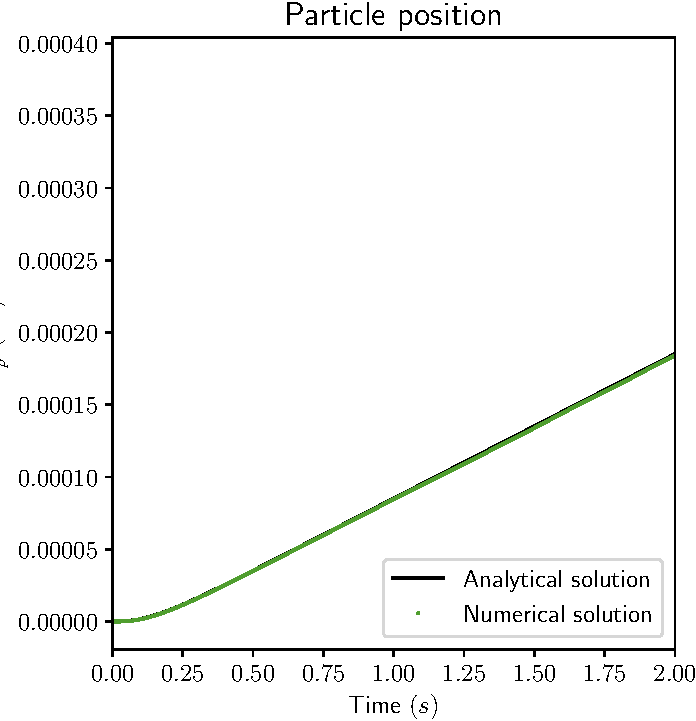
\includegraphics[width=0.48\textwidth]{\IMAGES/VNV/Fig_NUM_SCHEME_xp_xp_LIMIT_CASE_II.pdf}
  }
  \subfigure[{Particle velocity}]{
    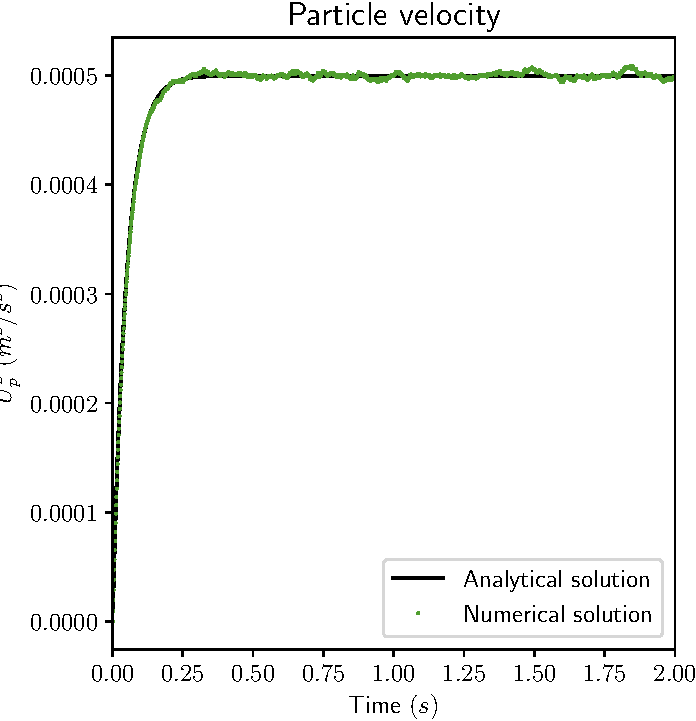
\includegraphics[width=0.48\textwidth]{\IMAGES/VNV/Fig_NUM_SCHEME_Up_Up_LIMIT_CASE_II.pdf}
  }
  \subfigure[{Fluid velocity seen}]{
    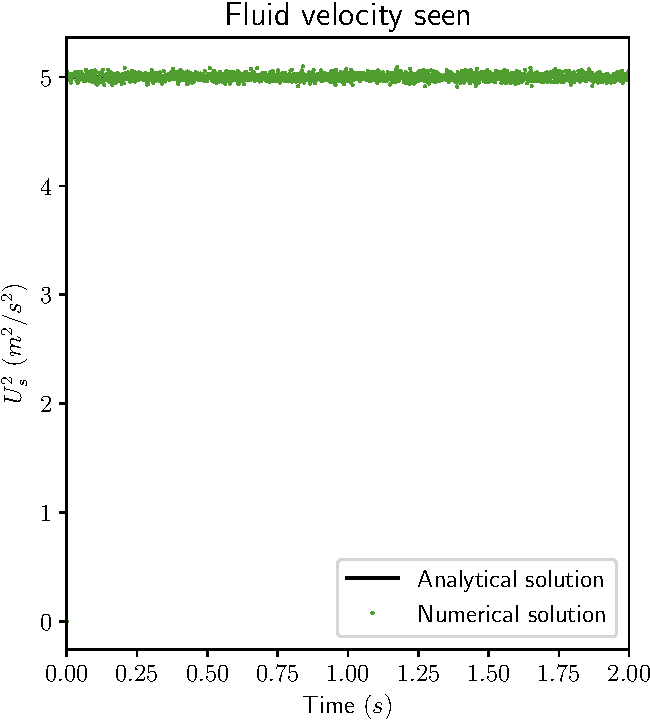
\includegraphics[width=0.48\textwidth]{\IMAGES/VNV/Fig_NUM_SCHEME_Us_Us_LIMIT_CASE_II.pdf}
  }
  \subfigure[{Velocity covariance}]{
    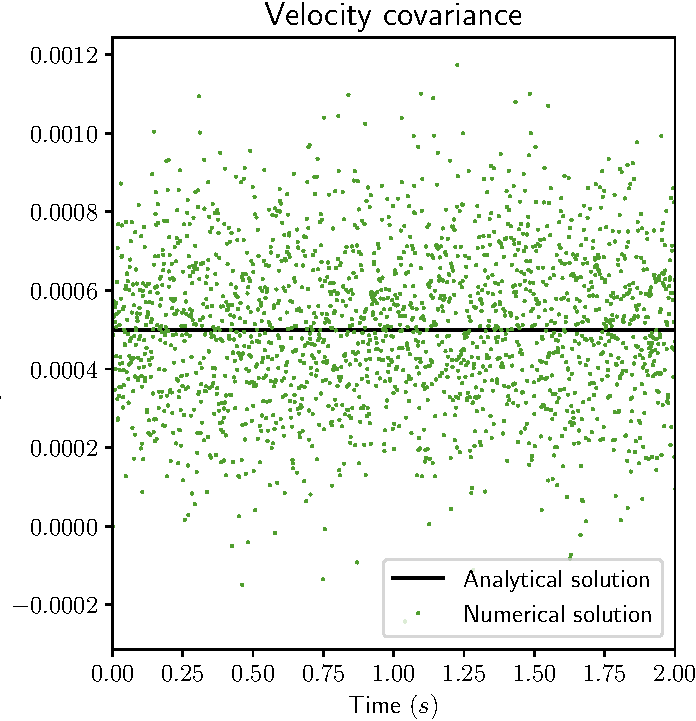
\includegraphics[width=0.48\textwidth]{\IMAGES/VNV/Fig_NUM_SCHEME_Up_Us_LIMIT_CASE_II.pdf}
  }
  \caption{Comparison of numerical results for system~\ref{eq:lagr:num_schem:syst} (symbols for $1^{st}$ and $2^{nd}$ order schemes) and analytical solutions (lines) in the limit case II.}
  \label{Fig_NUM_SCHEME_LIMIT_CASE_II}
\end{figure}

\begin{figure}[H]
  \centering
  \subfigure[{Position}]{
    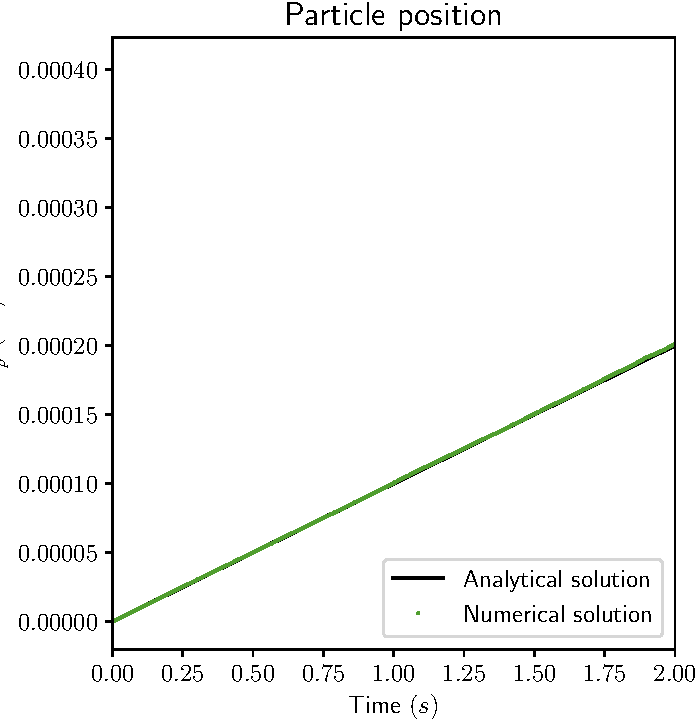
\includegraphics[width=0.48\textwidth]{\IMAGES/VNV/Fig_NUM_SCHEME_xp_xp_LIMIT_CASE_III.pdf}
  }
  \subfigure[{Particle velocity}]{
    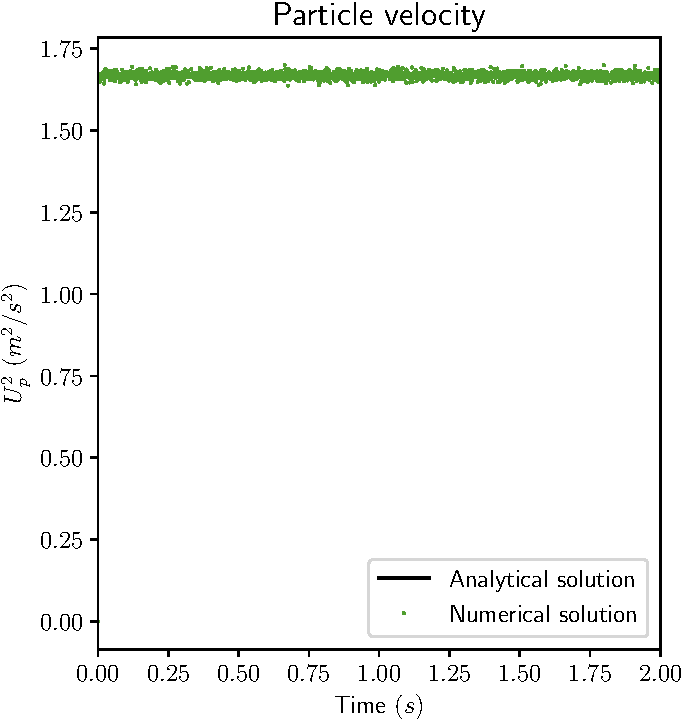
\includegraphics[width=0.48\textwidth]{\IMAGES/VNV/Fig_NUM_SCHEME_Up_Up_LIMIT_CASE_III.pdf}
  }
  \subfigure[{Fluid velocity seen}]{
    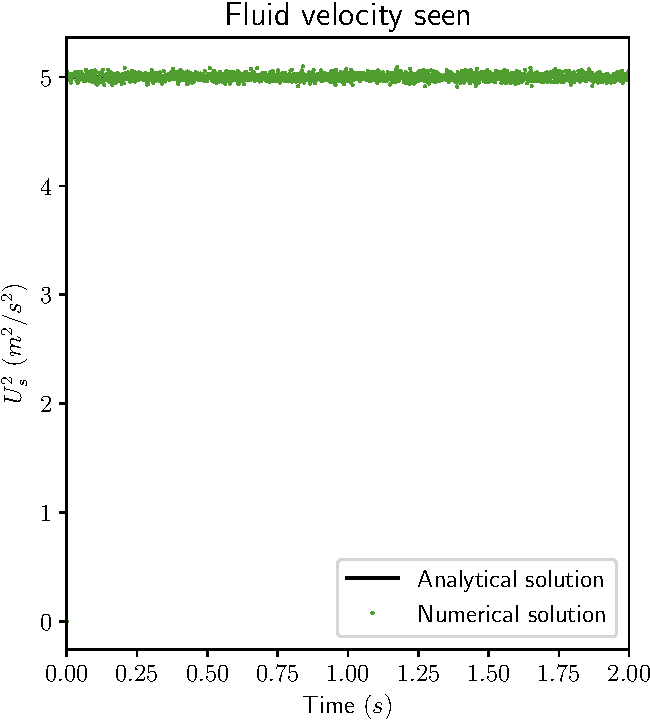
\includegraphics[width=0.48\textwidth]{\IMAGES/VNV/Fig_NUM_SCHEME_Us_Us_LIMIT_CASE_III.pdf}
  }
  \subfigure[{Velocity covariance}]{
    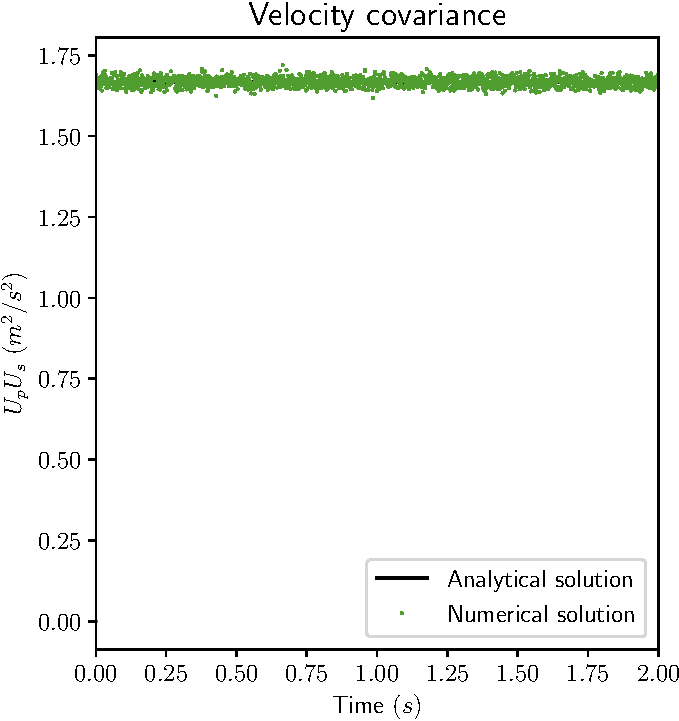
\includegraphics[width=0.48\textwidth]{\IMAGES/VNV/Fig_NUM_SCHEME_Up_Us_LIMIT_CASE_III.pdf}
  }
  \caption{Comparison of numerical results for system~\ref{eq:lagr:num_schem:syst} (symbols for $1^{st}$ and $2^{nd}$ order schemes) and analytical solutions (lines) in the limit case III.}
  \label{Fig_NUM_SCHEME_LIMIT_CASE_III}
\end{figure}


\section{Conclusions}
Overall, this algorithm for the numerical scheme is precise and robust even in all the ideal cases considered.

\clearpage

%%%%%%%%%%%%%%%%%%%%%%%%%%%%%%%%%%%%%%%%%%%%%%%%%%%%%%%%%
%                                                       %
%            End of test case desciption                %
%                                                       %
%%%%%%%%%%%%%%%%%%%%%%%%%%%%%%%%%%%%%%%%%%%%%%%%%%%%%%%%%

